\subsection{Elipsoide en la aproximación cuasiestática}
En esta sección se busca estudiar el esparcimiento de luz por un elipsoide centrado en el origen, con semiejes ($a,b,c$) paralelos a los ejes $\uvec{x},\uvec{y},\uvec{z}$ respectivamente, y con dimensiones tales que $\lambda\gg a>b>c$.\\


La partícula regular suave más general que cumple con lo anterior es un elipsoide con semiejes $a > b > c$, cuya superficie está dada por 
\begin{equation}
    \frac{x^2}{a^2}+\frac{y^2}{b^2}+\frac{z^2}{c^2}=1.
\end{equation}

Las coordenadas más naturales, aunque poco conocidas, para estudiar el sistema enunciado previamente son las coordenadas elipsoidales (ver Fig.). Introduciendo la familia de superficies confocales de segundo grado \cite{Math}
\begin{equation}
    \frac{x^2}{a^2+u}+\frac{y^2}{b^2+u}+\frac{z^2}{c^2+u}=1,
\end{equation}
donde $a>b>c$. La ecuación para calcular $u$ corresponde a un polinomio de tercer grado, por lo que tiene tres raíces reales diferentes $\xi,\eta,\zeta$, que se encuentran en los rangos
\begin{equation}
    -c^2<\xi<\infty,\hspace{0.5cm}-b^2<\eta<-c^2,\hspace{0.5cm}-a^2<\zeta<\infty
\end{equation}
por lo cual, 
\begin{align}
    \frac{x^2}{a^2+\xi}+\frac{y^2}{b^2+\xi}+\frac{z^2}{c^2+\xi}=1,&& -c^2<\xi<\infty;\\
    \frac{x^2}{a^2+\eta}+\frac{y^2}{b^2+\eta}+\frac{z^2}{c^2+\eta}=1,&& -b^2<\eta<-c^2;\\
    \frac{x^2}{a^2+\zeta}+\frac{y^2}{b^2+\zeta}+\frac{z^2}{c^2+\zeta}=1,&& -a^2<\zeta<-b^2.
\end{align}

donde ($\uvec{\xi},\uvec{\eta},\uvec{\zeta}$) corresponden al sistema de coordenadas elipsoidales  conveniente para la simetría del problema. Obsérvese que si $\xi$ es constante, se obtiene un elipsoide confocal. De esta forma, la superficie de la partícula a estudiar se tiene cuando $\xi=0$. Cuando $\eta$ es constante, se obtiene un hiperboloide de una hoja y cuando $\zeta$ es constante se tiene un hiperboloide de dos hojas.\\
\begin{figure}[H]
    \centering
    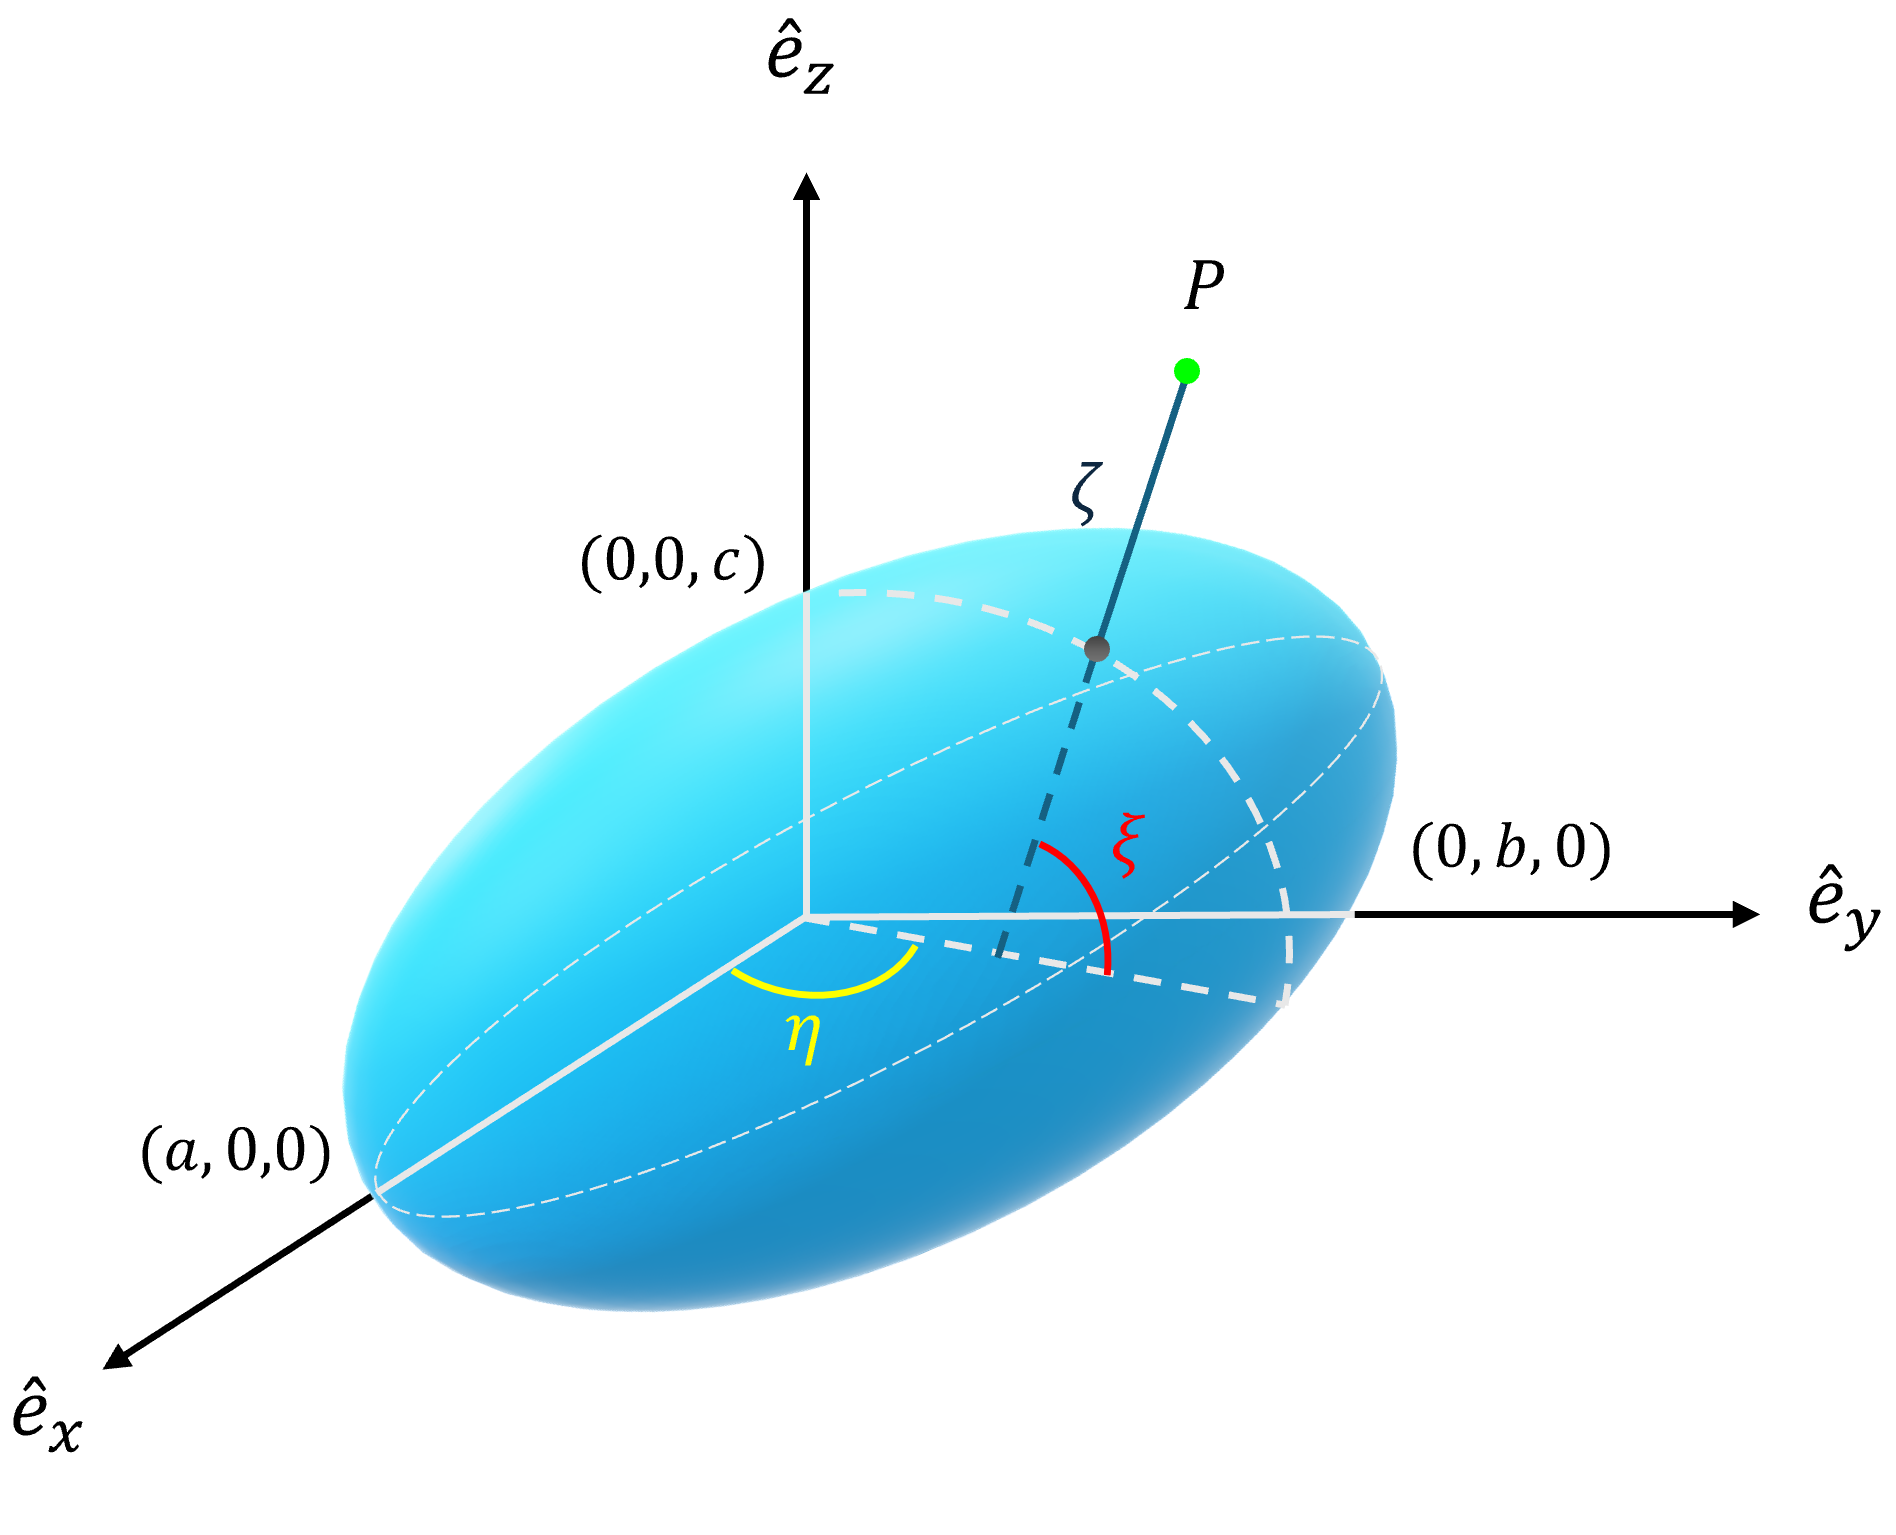
\includegraphics[width=9cm]{../../../../Pictures/servicio social/elipticalcoordinates.png} 
    \caption{Sistema coordenado elipsoidal con un elipsoide centrado en el origen, con semiejes ($a, b, c$), $a > b > c.$}
    \label{fig:enter-label}
\end{figure}

Las ecuaciones anteriores constituyen un sistema de ecuaciones que se puede expresar de forma matricial como

\begin{equation*}
    \begin{pmatrix}
    \frac{1}{a^2+\xi} & \frac{1}{b^2+\xi} & \frac{1}{c^2+\xi}\\
    \frac{1}{a^2+\eta} & \frac{1}{a^2+\eta} & \frac{1}{a^2+\eta}\\
    \frac{1}{a^2+\zeta} & \frac{1}{a^2+\zeta} & \frac{1}{a^2+\zeta}\end{pmatrix}\begin{pmatrix}
        x^2\\
        y^2\\
        z^2
    \end{pmatrix}=\begin{pmatrix}
        1\\
        1\\
    \end{pmatrix}
\end{equation*}
cuya solución se encontrará encontrando la inversa de la matriz anterior, que es \cite{Miguel}
\begin{equation*}
    \begin{pmatrix}
        \frac{(a^2+\xi)(b^2+\xi)(c^2+\xi)(a^2+\eta)(a^2+\zeta)}{(a^2-b^2)(a^2-c^2)(\xi-\eta)(\xi-\zeta)} & \frac{(a^2+\xi)(a^2+\eta)(b^2+\eta)(c^2+\eta)(a^2+\xi)}{(b^2-a^2)(a^2-c^2)(\zeta-\eta)(\eta-\zeta)} & -\frac{(a^2+\xi)(a^2+\eta)(a^2+\zeta)(b^2+\zeta)(c^2+\zeta)}{(a^2-b^2)(a^2-c^2)(\xi-\zeta)(\zeta-\eta)}\\
        \frac{(a^2+\xi)(b^2+\xi)(c^2+\xi)(b^2+\eta)(b^2+\zeta)}{(b^2-a^2)(b^2-c^2)(\xi-\eta)(\xi-\zeta)} &\frac{(c^2+\eta)(b^2+\zeta)(b^2+\xi)(b^2+\eta)(a^2+\eta)}{(b^2-c^2)(a^2-b^2)(\xi-\eta)(\eta-\zeta)} &\frac{(b^2+\xi)(b^2+\eta)(a^2+\zeta)(b^2+\zeta)(c^2+\zeta)}{(a^2-b^2)(b^2-c^2)(\xi-\zeta)(\zeta-\eta)}\\
        -\frac{(a^2+\xi)(b^2+\xi)(c^2+\xi)(c^2+\eta)(c^2+\zeta)}{(a^2-c^2)(c^2-b^2)(\xi-\eta)(\xi-\zeta)} & \frac{(c^2+\xi)(a^2+\eta)(b^2+\eta)(c^2+\eta)(c^2+\zeta)}{(a^2-c^2)(c^2-b^2)(\xi-\eta)(\eta-\zeta)} &
        \frac{(c^2+\xi)(c^2+\eta)(a^2+\zeta)(b^2+\zeta)(c^2+\zeta)}{(a^2-b^2)(c^2-b^2)(\xi-\zeta)(\zeta-\eta)}
    \end{pmatrix}
\end{equation*}.

Entonces, se tiene que

\begin{align}
    x^2&=\frac{(a^2+\xi)(a^2+\eta)(a^2+\zeta)}{(b^2-a^2)(c^2-a^2)},\label{def_x}\\
     y^2&=\frac{(b^2+\xi)(b^2+\eta)(b^2+\zeta)}{(a^2-b^2)(c^2-b^2)},\\
     z^2&=\frac{(c^2+\xi)(c^2+\eta)(c^2+\zeta)}{(a^2-c^2)(b^2-c^2)}.    
\end{align}

De esta forma, a cualquier punto ($x,y,z$) le corresponde un conjunto de coordenadas elipsoidales ($\xi,\eta,\zeta$). Sin embargo, esto no es cierto para el caso contrario. Estas coordenadas determinan ocho puntos simétricamente localizados en cada uno de los octantes cuyo espacio está particionado por los ejes coordenados $x,y,z$ anteriormente mencionados.\\

Consideremos un elipsoide homogéneo bajo un campo eléctrico incidente uniforme alineado a lo largo del eje $\uvec{z}$. El potencial tiene las propiedades de simetría
\begin{equation}
    \phi(x,y,z)=\phi(-x,y,z)=\phi(x,-y,z)=\phi(-x,-y,z),
\end{equation}
\begin{equation}
    \phi(x,y,-z)=\phi(-x,y,-z)=\phi(x,-y,-z)=\phi(-x,-y,-z),
\end{equation}
donde $x,y,z$ son positivas. Entonces, solo se tiene que considerar el potencial en dos octantes: uno con $z$ positivo y otro con $z$ negativo. Más aún, el potencial y su derivada con respecto a $z$ deben de ser continuos en el plano $z=0$. El campo incidente $\Vec{E}_0=E_0\uvec{z}$ se puede describir mediante el potencial como
\begin{equation}
\phi_0=-E_0 r\cos\theta=-E_0 z=-E_0\left[\frac{(c^2+\xi)(c^2+\eta)(c^2+\zeta)}{(a^2-c^2)(b^2-c^2)}\right]^{1/2}. 
\label{pot_0}
\end{equation}


Se debe de considerar un potencial de perturbación ($\phi_p$) asociado al esparcimiento producido por la partícula. En consecuencia, el potencial fuera de la partícula $\phi_{ext}$ está formado por la superposición del potencial incidente $\phi_0$ y el potencial de perturbación $\phi_p$
\begin{equation}
\phi_{ext}(\xi,\eta,\zeta)=\phi_0(\xi,\eta,\zeta)+\phi_p(\xi,\eta,\zeta).    
\end{equation}
Además, el potencial debe de ser continuo en la superficie de la elipse
\begin{equation}
\phi_{int}(0,\eta,\zeta)=\phi_{ext}(0,\eta,\zeta)+\phi_p(0,\eta,\zeta),    
\end{equation}
y, para distancias lo suficientemente lejanas a la partícula, es decir, cuando $\xi\gg a^2$, al factorizar $\xi$ de  la Ec.(\ref{def_x}), se tiene que 
\begin{equation*}
    \frac{x^2}{\frac{a^2}{\xi}+1}+\frac{y^2}{\frac{b^2}{\xi}+1}+\frac{z^2}{\frac{c^2}{\xi}+1}=\xi,
\end{equation*}
donde
\begin{equation*}
    \lim_{\xi\rightarrow\infty}\left(\frac{x^2}{\frac{a^2}{\xi}+1}+\frac{y^2}{\frac{b^2}{\xi}+1}+\frac{z^2}{\frac{c^2}{\xi}+1}\right)=x^2+y^2+z^2=r^2,
\end{equation*}
entonces, $\xi \simeq r^2$. Asimismo, en esta aproximación el potencial de perturbación es despreciable, por lo que 
\begin{equation}
\lim_{\xi\rightarrow\infty}\phi_p=0
\label{limitephi_p}.
\end{equation}

Sean $\phi_{int}$ y $\epsilon_1$ el potencial y la permitividad eléctrica en el interior del elipsoide y las mismas cantidades $\phi_{ext}$ y $\epsilon_m$ para el exterior de este, como el potencial es continuo y la componente tangencial del campo eléctrico también
\begin{subequations}
\label{condicionesfrontera}
\begin{align}
    \phi_{int}&=\phi_{ext}\label{cf1},\\
    \epsilon_1\frac{\partial \phi_{int}}{\partial \xi}\Big |_{\xi=0}&=
    \epsilon_m\frac{\partial \phi_{ext}}{\partial \xi}\Big |_{\xi=0}\label{cf2}.
\end{align}
\end{subequations}
Para resolver el sistema de ecuaciones anterior se necesita hacer un cambio de base de un sistema a otro. Para ello, se debe de encontrar un vector unitario en la dirección de la coordenada $i$, que mide cómo es que cambia el vector posición en una dirección dada y se define como \cite{Arfken}
\begin{equation}
    \uvec{i}=\frac{1}{h_i}\left(\frac{\partial \Vec{r}}{\partial q_i}\right), \hspace{0.5cm} i=1,2,3;    
\end{equation}
donde $h_i$ es el factor de escala
\begin{equation}
    h_i=\Big|\frac{\partial \Vec{r}}{\partial q_i}\Big|=\sqrt{\left(\frac{\partial x}{\partial q_i}\right)^2+\left(\frac{\partial y}{\partial q_i}\right)^2+\left(\frac{\partial z}{\partial q_i}\right)^2}.
\end{equation}
Por un lado, se tiene que 
\begin{align*}
  \frac{\partial x}{\partial \xi}&=\frac{1}{2}\left(\frac{(a^2+\xi)(a^2+\eta)(a^2+\zeta)}{(b^2-a^2)(c^2-a^2)}\right)^{-1/2}\frac{\partial}{\partial \xi}\left(\frac{(a^2+\xi)(a^2+\eta)(a^2+\zeta)}{(b^2-a^2)(c^2-a^2)}\right)\nonumber\\
  &=\frac{1}{2x}\frac{\partial x^2}{\partial\xi}=\frac{1}{2}\frac{1}{a^2+\xi}\sqrt{\frac{(a^2+\xi)(a^2+\eta)(a^2+\zeta)}{(b^2-a^2)(c^2-a^2)}}=\frac{1}{2}\frac{x}{(a^2+\xi)}
\end{align*}
por tanto,
\begin{equation}
    \frac{\partial x}{\partial \xi}=\frac{1}{2x}\frac{\partial x^2}{\partial\xi}=\frac{1}{2}\frac{x}{(a^2+\xi)}.
\end{equation}
Análogamente, para $y$ y $z$
\begin{align}
    \frac{\partial y}{\partial \xi}&=\frac{1}{2y}\frac{\partial y^2}{\partial\xi}=\frac{1}{2}\frac{y}{(b^2+\xi)},\\
    \frac{\partial z}{\partial \xi}&=\frac{1}{2z}\frac{\partial z^2}{\partial\xi}=\frac{1}{2}\frac{z}{(c^2+\xi)},
\end{align}
entonces, se tiene que el cuadrado del primer factor de escala $h_1$ es
\begin{equation}
    h_1^2=\frac{1}{4}\left[\frac{x^2}{(a^2+\xi)^2}+\frac{y}{(b^2+\xi)^2}+\frac{z}{(c^2+\xi)^2}\right].
    \label{h1}
\end{equation}
Por otro lado, se propone que
\begin{equation}
    1-\frac{x^2}{a^2+u}-\frac{y^2}{b^2+u}-\frac{z^2}{c^2+u}=\frac{g(u)}{(a^2+u)(b^2+u)(c^2+u)},
\end{equation}
donde $g(u)$ es una función cúbica con tres raíces reales dentro del rango descrito por las limitaciones de cada variable. Considerando la función $g(u)=(u-\xi)(u-\eta)(u-\zeta)$,  al derivar la ecuación anterior con respecto de $u$ se tiene que
\begin{align}
    \frac{x^2}{(a^2+u)^2}+\frac{y^2}{(b^2+u)^2}+\frac{z^2}{(c^2+u)^2}&=\frac{g(u)}{[f(u)]^2}\left[\frac{1}{u-\xi}+\frac{1}{u-\zeta}+\frac{1}{u-\eta}-\left(\frac{1}{a^2+u}+\frac{1}{b^2+u}+\frac{1}{c^2+u}\right)\right],
\end{align}
con 
\begin{equation}
    f(u)=\sqrt{(a^2+u)(b^2+u)(c^2+u)}.    
\end{equation}
De esta forma, se puede reescribir al primer factor de escala de la Ec.(\ref{h1}) como
\begin{align*}
h_1^2&=\frac{1}{4}\frac{g(u)}{[f(u)]^2}\left[\frac{1}{u-\xi}+\frac{1}{u-\zeta}+\frac{1}{u-\eta}-\left(\frac{1}{a^2+u}+\frac{1}{b^2+u}+\frac{1}{c^2+u}\right)\right]\nonumber\\
&=\frac{1}{4}\frac{g(u)}{[f(u)]^2}\left[\frac{(u-\zeta)(u-\eta)+(u-\xi)(u-\eta)+(u-\xi)(u-\zeta)}{g(u)}-\left(\frac{1}{a^2+u}+\frac{1}{b^2+u}+\frac{1}{c^2+u}\right)\right].    
\end{align*}
Considerando $u\rightarrow\xi$, $g(u)\rightarrow 0$, se tiene que el factor de escala $h_1$ es
\begin{equation}
    h_1=\frac{\sqrt{(\xi-\eta)(\xi-\zeta)}}{2f(\xi)}    
\end{equation}
análogamente, 
\begin{equation}
    h_2=\frac{\sqrt{(\eta-\xi)(\eta-\zeta)}}{2f(\eta)}
\end{equation}
y 
\begin{equation}
    h_3=\frac{\sqrt{(\zeta-\xi)(\zeta-\eta)}}{2f(\zeta)}
\end{equation}

El laplaciano en coordenadas generalizadas es \cite{Arfken}
\begin{equation}
    \nabla^2\phi=\frac{1}{h_1h_2h_3}\left[\frac{\partial}{\partial q_1}\left(\frac{h_2h_3}{h_1}\frac{\partial\phi}{\partial q_1}\right)+\frac{\partial}{\partial q_2}\left(\frac{h_3h_1}{h_2}\frac{\partial\phi}{\partial q_2}\right)+\frac{\partial}{\partial q_3}\left(\frac{h_1h_2}{h_3}\frac{\partial\phi}{\partial q_3}\right)\right],    
\end{equation}
donde $\phi$ es un escalar invariante. Por lo tanto, el laplaciano en coordenadas elipsoidales es
\begin{multline*}
    \nabla^2 \phi=\frac{1}{\frac{\sqrt{(\xi-\eta)(\xi-\zeta)}}{2f(\xi)}\frac{\sqrt{(\eta-\xi)(\eta-\zeta)}}{2f(\eta)}\frac{\sqrt{(\zeta-\xi)(\zeta-\eta)}}{2f(\zeta)}}\Bigg[\frac{\partial}{\partial\xi}\left(\frac{\frac{\sqrt{(\eta-\xi)(\eta-\zeta)}}{2f(\eta)}\frac{\sqrt{(\zeta-\xi)(\zeta-\eta)}}{2f(\zeta)}}{\frac{\sqrt{(\xi-\eta)(\xi-\zeta)}}{2f(\xi)}}\frac{\partial\phi}{\partial\xi}\right)\\+\frac{\partial}{\partial \eta}\left(\frac{\frac{\sqrt{(\zeta-\xi)(\zeta-\eta)}}{2f(\zeta)}\frac{\sqrt{(\xi-\eta)(\xi-\zeta)}}{2f(\xi)}}{\frac{\sqrt{(\eta-\xi)(\eta-\zeta)}}{2f(\eta)}}\frac{\partial\phi}{\partial\eta}\right)\\
    +\frac{\partial}{\partial \zeta}\left(\frac{\frac{\sqrt{(\xi-\eta)(\xi-\zeta)}}{2f(\xi)}\frac{\sqrt{(\eta-\xi)(\eta-\zeta)}}{2f(\eta)}}{\frac{\sqrt{(\zeta-\xi)(\zeta-\eta)}}{2f(\zeta)}}\frac{\partial\phi}{\partial\zeta}\right)\Bigg].
\end{multline*}
Sea $\Lambda=\frac{\sqrt{(\xi-\eta)(\xi-\zeta)(\eta-\xi)(\eta-\zeta)(\zeta-\xi)(\eta-\zeta)}}{8f(\xi)f(\eta)f(\zeta)}$,
\begin{multline*}
    \nabla^2\phi=\frac{\sqrt{(\eta-\zeta)(\zeta-\eta)}}{2\Lambda f(\eta)f(\zeta)}\frac{\partial}{\partial\xi}\left(f(\xi)\frac{\partial\phi}{\partial\xi}\right)+\frac{\sqrt{(\zeta-\xi)(\xi-\zeta)}}{2\Lambda f(\zeta)f(\xi)}\frac{\partial}{\partial\eta}\left(f(\eta)\frac{\partial\phi}{\partial\eta}\right)\\+\frac{\sqrt{(\xi-\eta)(\eta-\xi)}}{2\Lambda f(\eta)f(\xi)}\frac{\partial}{\partial\zeta}\left(f(\zeta)\frac{\partial\phi}{\partial\zeta}\right),
\end{multline*}
y que simplificando es
\begin{align}
    \nabla^2\phi&=\frac{4f(\xi)}{(\xi-\eta)(\zeta-\xi)}\frac{\partial}{\partial\xi}\left(f(\xi)\frac{\partial\phi}{\partial\xi}\right)+\frac{4f(\eta)}{(\xi-\eta)(\eta-\zeta)}\frac{\partial}{\partial\eta}\left(f(\eta)\frac{\partial\phi}{\partial\eta}\right)+\frac{4f(\zeta)}{(\zeta-\xi)(\eta-\xi)}\frac{\partial}{\partial\zeta}\left(f(\zeta)\frac{\partial\phi}{\partial\zeta}\right)\nonumber\\
    &=\frac{4}{\Upsilon}\left[(\eta-\zeta)f(\xi)\frac{\partial}{\partial\xi}\left(f(\xi)\frac{\partial\phi}{\partial\xi}\right)+(\zeta-\xi)f(\eta)\frac{\partial}{\partial\eta}\left(f(\eta)\frac{\partial\eta}{\partial\eta}\right)+(\xi-\zeta)f(\zeta)\frac{\partial}{\partial\zeta}\left(f(\zeta)\frac{\partial\phi}{\partial\zeta}\right)\right],
\end{align}
donde a $\Upsilon$ se le conoce como el valor absoluto del determinante funcional \cite{Kellogg}
\begin{equation}
    \Upsilon=(\xi-\eta)(\zeta-\xi)(\eta-\zeta).
\end{equation}
Como resultado de lo anterior, la ecuación de Laplace en coordenadas elipsoidales es
\begin{equation}
    \nabla^2\phi=(\eta-\zeta)f(\xi)\frac{\partial}{\partial\xi}\left(f(\xi)\frac{\partial\phi}{\partial\xi}\right)+(\zeta-\xi)f(\eta)\frac{\partial}{\partial\eta}\left(f(\eta)\frac{\partial\eta}{\partial\eta}\right)+(\xi-\eta)f(\zeta)\frac{\partial}{\partial\zeta}\left(f(\zeta)\frac{\partial\phi}{\partial\zeta}\right)=0
    \label{laplaceplisoidal}
\end{equation}
Esta ecuación no es sencilla de resolver a pesar de ser considerablemente simétrica. Para resolverla se podría proponer hacerlo por el método de separación de variables y así expandir al potencial real como una suma de armónicos  elipsoidales, pero como la solución a esta ecuación está determinada por la forma del campo
incidente, que a su vez está descrito por el potencial anterior, y que necesariamente cumple las condiciones de contorno, se buscará resolver mediante el método de reducción de orden proponiendo una solución no trivial y buscar una segunda solución como se verá a continuación.\\

En la Ec.(\ref{pot_0}) se propuso a los potenciales $\phi_{int}$ y $\phi_p$ de la forma
\begin{align}
    \phi_0(\xi,\eta,\zeta)&=-E_0\left[\frac{(c^2+\xi)(c^2+\eta)(c^2+\zeta)}{(a^2-c^2)(b^2-c^2)}\right]^{1/2}\nonumber\\
    &=F(\xi)[(c^2+\eta)(c^2+\zeta)]^{1/2}
    \label{phi0 con F}
\end{align}
los cuales tienen que satisfacer la Ec. (\ref{laplaceplisoidal}). Por un lado, 
\begin{align}
     (\eta-\zeta)f(\xi)\frac{\partial}{\partial\xi}\left(f(\xi)\frac{\partial\phi}{\partial\xi}\right)&= (\eta-\zeta)[(c^2+\eta)(c^2+\zeta)]^{1/2}\left[f(\xi)\frac{d}{d\xi}\left(f(\xi)\frac{ d F(\xi)}{d\xi}\right)\right],\label{laplace1}
\end{align}
y,
\begin{align}
    (\zeta-\xi)f(\eta)\frac{\partial}{\partial\eta}\left(f(\eta)\frac{\partial\phi}{\partial\eta}\right)&=(\zeta-\xi)F(\xi)(c^2+\zeta)^{1/2}\left[f(\eta)\frac{\partial}{\partial\eta}\left(f(\eta)\frac{\partial}{\partial\eta}(c^2+\eta)^{1/2}\right)\right]\nonumber\\
    &=\frac{1}{4}(\zeta-\xi)[(c^2+\zeta)(c^2+\eta)^{1/2}(a^2+b^2+2\eta)F(\xi).\label{laplace2}
\end{align}
Análogamente,
\begin{equation}
    (\xi-\eta)f(\zeta)\frac{\partial}{\partial\zeta}\left(f(\zeta)\frac{\partial\phi}{\partial\zeta}\right)=\frac{1}{4}(\xi-\eta)[(c^2+\zeta)(c^2+\eta)]^{1/2}(a^2+b^2+2\zeta)F(\xi).\label{laplace3}
\end{equation}
Sumando las Ecs.(\ref{laplace1}), (\ref{laplace2}) y (\ref{laplace3}) 
\begin{equation}
  (\eta-\zeta)[(c^2+\zeta)(c^2+\eta)]^{1/2}\left[f(\xi)\frac{d}{d\xi}\left(f(\xi)\frac{ d F(\xi)}{d\xi}\right)-\frac{1}{4}F(\xi)(a^2+b^2+2\xi)\right]=0,
\end{equation}
por lo que para que se satisfaga la Ec.(\ref{laplaceplisoidal}) basta que
\begin{equation}
    f(\xi)\frac{d}{d\xi}\left(f(\xi)\frac{ d F(\xi)}{d\xi}\right)-\left(\frac{a^2+b^2}{4}+\frac{\xi}{2}\right)F(\xi)=0.
\end{equation}
Existen dos soluciones linealmente independientes a la ecuación diferencial (ordinaria) anterior. Se propone
la primera solución como
\begin{equation}
    F_1(\xi)=(c^2+\xi)^{1/2},
    \label{F1}
\end{equation}
y la segunda solución se obtendrá mediante el método de reducción de orden. Como $F_1(\xi)$ es solución de la Ec.(\ref{F1}), entonces también 
$F_2(\xi)=v(\xi)F_1(\xi)$ lo es. Derivando la ecuación anterior respecto a $\xi$
\begin{align}
    \frac{dF_2(\xi)}{d\xi}&=F_1(\xi)\frac{dv(\xi)}{d\xi}+v(\xi)\frac{F_1(\xi)}{d\xi},\\
    \frac{d^2F_2(\xi)}{d\xi^2}&=F_1(\xi)\frac{d^2v(\xi)}{d\xi^2}+2\frac{dv(\xi)}{d\xi}\frac{dF_1(\xi)}{d\xi}+v(\xi)\frac{d^2F_1(\xi)}{d\xi^2},
\end{align}
y sustituyendo las derivadas anteriores en la Ec.(\ref{F1}), se obtiene
\begin{multline}
    f^2(\xi)\left(F_1(\xi)\frac{d^2v(\xi)}{d\xi^2}+2\frac{dv(\xi)}{d\xi}\frac{dF_1(\xi)}{d\xi}+\cancel{v(\xi)\frac{d^2F_1(\xi)}{d\xi^2}}\right)\\+\left(F_1(\xi)\frac{dv(\xi)}{d\xi}+\cancel{v(\xi)\frac{F_1(\xi)}{d\xi}}\right)f(\xi)\frac{df(\xi)}{d\xi}-
    \\ \cancel{\left(\frac{a^2+b^2}{4}+\frac{\xi}{2}\right)v(\xi)F_1(\xi)}=0,
\end{multline}
de donde tres términos se eliminan, pues
\begin{equation*}
    v(\xi)\frac{d^2F_1(\xi)}{d\xi^2}f^2(\xi)=-\frac{1}{4}v(\xi)[(a^2+\xi)(b^2+\xi)(c^2+\xi)^{-1/2}]
\end{equation*}
\begin{multline*}
    v(\xi)\frac{dF_1(\xi)}{d\xi}f(\xi)\frac{df(\xi)}{d\xi}=\frac{1}{4}v(\xi)(a^2+\xi)(b^2+\xi)(c^2+\xi)^{-1/2}+\left(\frac{a^2+b^2}{4}+\frac{\xi}{2}\right)v(\xi)F_1(\xi)\\-\left(\frac{a^2+b^2}{4}+\frac{\xi}{2}\right)v(\xi)F_1(\xi),
\end{multline*}
es así como
\begin{equation*}
    f^2(\xi)F_1(\xi)\frac{d^2v(\xi)}{d\xi^2}+\frac{dv(\xi)}{d\xi}\left[f(\xi)F_1(\xi)\frac{df(\xi)}{d\xi}+2f^2(\xi)\frac{dF_1(\xi)}{d\xi}\right]=0.
\end{equation*}
Haciendo el cambio de variable $V(\xi)=dv(\xi)/d\xi$, se tiene que
\begin{equation*}
    f^2(\xi)F_1(\xi)\frac{dV(\xi)}{d\xi^2}+V(\xi)\left[f(\xi)F_1(\xi)\frac{df(\xi)}{d\xi}+2f^2(\xi)\frac{dF_1(\xi)}{d\xi}\right]=0,    
\end{equation*}
\begin{equation*}
    \frac{1}{V(\xi)}\frac{dV(\xi)}{d\xi}=-\frac{1}{f^2(\xi)F_1(\xi)}\left[f(\xi)F_1(\xi)\frac{df(\xi)}{d\xi}+2f^2(\xi)\frac{dF_1(\xi)}{d\xi}\right].
\end{equation*}
Integrando la ecuación anterior se obtiene
\begin{align}
    ln[V(q)]=\int^{q}\frac{1}{V(\xi)}dV(\xi)&=-\left[\int^q \frac{df(\xi)}{f(\xi)}+2\int^q \frac{dF_1(\xi)}{F_1(\xi)}\right]\nonumber\\
    &=-\{ln[f(q)]+ln[F_1^2(q)]\}=-ln[F_1^2(q)f(q)],
\end{align}
entonces,
\begin{equation}
    \frac{dv(q)}{dq}=\frac{1}{F_1^2(q)f(q)},
\end{equation}
donde $dv(q)/dq\neq 0$, por lo que $v(q)\neq $constante. Integrando lo anterior se tiene que
\begin{equation}
    v(\xi)=\int_{\xi}^{\infty}\frac{dq}{F_1^2(q)f(q)},
\end{equation}
por lo tanto, 
\begin{equation}
  F_2(\xi)=F_1(\xi)\int_{\xi}^{\infty}\frac{dq}{F_1^2(q)f(q)},
  \label{F2}
\end{equation}
donde, en principio, los límites de integración son arbitrarios; sin embargo se han elegido los que aparecen
en la Ec.(\ref{F2}), pues al escribir explícitamente el integrando, usando las Ecs. (\ref{F1}) y (\ref{F2}), se obtiene
\begin{align}
    F_2(\xi)&=F_1(\xi)\int_{\xi}^{\infty}\frac{dq}{(c^2+q)[(a^2+q)(b^2+q)(c^2+q)]^{1/2}}\nonumber\\
    &=\frac{2F_1(\xi)}{c^2-b^2}\Bigg\{\left[\frac{b^2+q}{(a^2+q)(c^2+q)}\right]^{1/2}-\frac{1}{(a^2-c^2)^{1/2}}E\left(\mbox{arcsen}\left(\frac{\sqrt{a^2-c^2}}{a^2+q}\right)\Bigg|\frac{a^2-b^2}{a^2-c^2}\right)\Bigg\}\Bigg|_0^{\infty},
\end{align}
donde $E(\phi|k)$ es una integral elíptica de segundo orden definida como \cite{Abramo}
\begin{equation}
    E(x|m)=\int_{0}^x\frac{\sqrt{1-mt^2}}{1-t^2}dt,\hspace{1cm}0\leq m\leq 1,
\end{equation}
donde el parámetro $m$ se define como $m\equiv k^2$, el módulo angular es $\alpha=\mbox{arcsin}\:k$ y $\varphi$ es la amplitud que cumple $x=\sin\varphi$. En el primer límite de integración ($\infty$) de $F_2(\xi)$ al evaluar se obtiene que el primer sumando es cero, y en el segundo la función arcoseno es cero. De esta forma, la parte angular de la integral es cero, es decir, $E(0|m)=0$. En consecuencia, considerando la definición de $F_1$ en la Ec.(\ref{F1}) se tiene que $F_1$ y $F_2$ cumplen

\begin{equation}
    \lim_{\xi \to 0}F_1(\xi)=c\hspace{1cm}\mbox{y}\hspace{1cm} \lim_{\xi \to \infty}F_2(\xi)=0.
\end{equation}
De esta forma, los potenciales $\phi_{int}$ y $\phi_p$, propuestos como en la Ec.(\ref{phi0 con F}), considerando que $F_1$ no satisface la condición impuesta sobre $\phi_p$ en la Ec. (\ref{limitephi_p}) y que el potencial dentro de la partícula debe de ser finito y $F_2$ no cumple con esto, están dados por
\begin{align}
    \phi_{int}&=C_1F_1(\xi)[(c^2+\eta)(c^2+\zeta)]^{1/2}\label{phi_int},\\
    \phi_p&=C_2F_2(\xi)[(c^2+\eta)(c^2+\zeta)]^{1/2}\label{phi_p},
\end{align}
donde $C_1$ y $C_2$ son constantes determinadas a partir de las condiciones de frontera dadas por las Ecs.(\ref{condicionesfrontera}). Usando la primera condición de contorno de la Ec.(\ref{cf1}), se tiene que,
\begin{equation}
    C_1F_1(\xi)[(c^2+\eta)(c^2+\zeta)]^{1/2}=E_0\left[\frac{(c^2+\xi)(c^2+\eta)(c^2+\zeta)}{(a^2-c^2)(b^2-c^2)}\right]^{1/2}+C_2F_2(\xi)[(c^2+\eta)(c^2+\zeta)]^{1/2}
\end{equation}
entonces, 
\begin{align}
    C_1F_1(\xi)&=E_0\left[\frac{(c^2+\xi)}{(a^2-c^2)(b^2-c^2)}\right]^{1/2}+C_2F_2(\xi)\nonumber\\
    \Rightarrow \frac{C_2F_2(\xi)-C_1F_1(\xi)}{(c^2+\xi)^{1/2}}&=\frac{E_0}{[(a^2-c^2)(b^2-c^2)]^{1/2}}\nonumber\\
    \Rightarrow \frac{C_2 F_1(\xi)\int_{0}^{\infty}\frac{dq}{(c^2+q)f(q)}-C_1F_1(\xi)}{(c^2+\xi)^{1/2}}&=\frac{E_0}{[(a^2-c^2)(b^2-c^2)]^{1/2}}\nonumber\\
    \Rightarrow C_2 \int_{0}^{\infty}\frac{dq}{(c^2+q)f(q)}-C_1&=\frac{E_0}{[(a^2-c^2)(b^2-c^2)]^{1/2}}.
\end{align}
Si definimos
\begin{equation}
    L^{(3)}=\frac{abc}{2}\int_{0}^{\infty}\frac{dq}{(c^2+q)f(q)},
\end{equation}
entonces,
\begin{equation}
    C_2L^{(3)}\left(\frac{2}{abc}\right)-C_1=\frac{E_0}{[(a^2-c^2)(b^2-c^2)]^{1/2}}
    \label{ec1 de cf}
\end{equation}
Usando la segunda condición de contorno de la Ec.(\ref{cf2}), se tiene que
\begin{multline*}
    \frac{\epsilon_1C_1}{2}\left[\frac{(c^2+\eta)(c^2+\zeta)}{(c^2+\xi)}\right]^{1/2}=\frac{\epsilon_mE_0}{2}\left[\frac{(c^2+\eta)(c^2+\zeta)}{(c^2+\xi)(a^2-c^2)(b^2-c^2)}\right]^{1/2}+\frac{\epsilon_m C_2}{2}\left[\frac{(c^2+\eta)(c^2+\zeta)}{(c^2+\xi)}\right]^{1/2}\int_{\xi}^{\infty}\frac{dq}{(c^2+q)f(q)}\\
    +\epsilon_mC_2[(c^2+\xi)(c^2+\eta)(c^2+\zeta)]^{1/2}\frac{d}{d\xi}\Bigg\{\int_{\xi}^{\infty}\frac{dq}{(c^2+q)f(q)}\Bigg\},
\end{multline*}
donde la integral del tercer sumando es
\begin{align*}
    \frac{d}{d\xi}\left[\int_{\xi}^{\infty}\frac{dq}{(c^2+q)f(q)}\right]&=\frac{d}{d\xi}\left[\lim_{a\to\infty}\int_{\xi}^{a}\frac{dq}{(c^2+q)f(q)}\right]=-\lim_{a\to\infty}\frac{1}{(c^2+\xi)f(\xi)}=-\frac{1}{(c^2+\xi)f(\xi)}.
\end{align*}
Al evaluar en $\xi=0$ se tiene que
\begin{align*}
    \frac{\epsilon_1C_1}{2}&=\epsilon_m E_0\left[\frac{1}{(a^2-c^2)(b^2-c^2)}\right]^{1/2}+\epsilon_m C_2\left(\frac{2}{abc}\right)\left(L^{(3)}-1\right),
\end{align*}
por tanto,
\begin{equation}
    \epsilon_m C_2\left(\frac{2}{abc}\right)\left(L^{(3)}-1\right)- \epsilon_1 C_1=\frac{\epsilon_m E_0}{[(a^2-c^2)(b^2-c^2)]^{1/2}}.
     \label{ec2 de cf}
\end{equation}
Las constantes $C_1$ y $C_2$ se obtienen de resolver el sistema de ecuaciones entre las Ecs. (\ref{ec1 de cf}) y (\ref{ec2 de cf}), por lo
cual, al multiplicar la Ec. (\ref{ec1 de cf}) por $\epsilon_1$ menos la Ec.(\ref{ec2 de cf})
\begin{equation*}
    \epsilon_1C_2L^{(3)}\left(\frac{2}{abc}\right)-C_1\epsilon_1-\epsilon_m C_2\left(\frac{2}{abc}\right)\left(L^{(3)}-1\right)- \epsilon_1 C_1=\epsilon_1\frac{E_0}{[(a^2-c^2)(b^2-c^2)]^{1/2}}-\frac{\epsilon_m E_0}{[(a^2-c^2)(b^2-c^2)]^{1/2}},
\end{equation*}
simplificando se obtiene que
\begin{equation}
    C_2=\frac{abc}{2}\frac{E_0(\epsilon_1-\epsilon_m)}{[(a^2-c^2)(b^2-c^2)]^{1/2}}\left[L^{(3)}(\epsilon_1-\epsilon_m)+\epsilon_m\right]^{-1},
\end{equation}
por lo tanto, al sustituir $C_2$ en la Ec.(\ref{ec1 de cf}) se tiene que:
\begin{equation}
    C_1=\frac{E_0}{[(a^2-c^2)(b^2-c^2)]^{1/2}}\Bigg\{ \left[1+\frac{\epsilon_m}{L^{(3)}(\epsilon_1-\epsilon_m)}\right]^{-1}-1\Bigg\}.
\end{equation}
De esta forma, ya se puede determinar el potencial dentro de la partícula sustituyendo $F_1$ y $C_1$ en la Ec.(\ref{phi_int}), por lo que
\begin{align}
    \phi_{int}&=E_0\left[\frac{(c^2+\xi)(c^2+\eta)(c^2+\zeta)}{(a^2-c^2)(b^2-c^2)}\right]^{1/2}\Bigg\{ \left[1+\frac{\epsilon_m}{L^{(3)}(\epsilon_1-\epsilon_m)}\right]^{-1}-1\Bigg\}\nonumber\\
    &=\phi_0 \left[\frac{\epsilon_m}{L^{(3)}(\epsilon_1-\epsilon_m)+\epsilon_m}\right]\nonumber\\
    &=\frac{1}{1+\frac{L^{(3)}(\epsilon_1-\epsilon_m)}{\epsilon_m}}\phi_0
\end{align}
y,
\begin{equation}
    \phi_p=\frac{abc}{2}\frac{\frac{(\epsilon_m-\epsilon_1)}{\epsilon_m}\int_{\xi}^{\infty}\frac{dq}{F_1^2(q)f(q)}}{1+\frac{L^{(3)}(\epsilon_1-\epsilon_m)}{\epsilon_m}}\phi_0.
\end{equation}

A pesar de que inicialmente se había considerado el octante donde $x,y,z$ eran positivas, las ecuaciones anteriormente obtenidas nos dan el potencial en todos los puntos del espacio, como consecuencia de la simetría de la partícula.\\

Si consideramos distancias $r$ muy alejadas del origen tales que $\xi\simeq r^2\gg a^2$ se tiene que
\begin{equation*}
    \int_{\xi}^{\infty}\frac{dq}{F_1^2(q)f(q)}= \int_{\xi}^{\infty}\frac{dq}{(c^2+q)f(q)}=\int_{\xi}^{\infty}\frac{dq}{q^{5/2}}=\frac{2}{3}\xi^{-3/2},
\end{equation*}
y entonces el potencial $\phi_p$ está dado por
\begin{equation}
    \phi_p\sim\frac{E_0\cos\theta}{r^2}\frac{\frac{abc}{3}\frac{\epsilon_1-\epsilon_m}{\epsilon_m}}{1+\frac{L^{(3)}(\epsilon_1-\epsilon_m)}{\epsilon_m}},\hspace{1cm}(r\gg a)
\end{equation}
que identificamos como el potencial de un dipolo eléctrico con momento 
\begin{equation}
    \Vec{p}=4\pi\epsilon_m abc\frac{\epsilon_1-\epsilon_m}{3\epsilon_m+3L^{(3)}(\epsilon_1-\epsilon_m)}\Vec{E}_0
    \label{momento_dip}.
\end{equation}
Entonces, la polarizabilidad $\alpha_3$ de un elipsoide en un campo paralelo a uno de sus ejes principales es
\begin{equation}
    \alpha^{(3)}=V\frac{\epsilon_1-\epsilon_m}{\epsilon_m+L^{(3)}(\epsilon_1-\epsilon_m)},
\end{equation}
donde $V=4\pi abc/3$ es el volumen del elipsoide. Siguiendo con esta idea, las polarizabilidades $\alpha_1$ y $\alpha_2$ cuando el campo es aplicado en los ejes $x$ y $y$ son:
\begin{align}
    \alpha^{(1)}&=4\pi abc \frac{\epsilon_1-\epsilon_m}{3\epsilon_m+3L^{(1)}(\epsilon_1-\epsilon_m)},\\
    \alpha^{(2)}&=4\pi abc \frac{\epsilon_1-\epsilon_m}{3\epsilon_m+3L^{(2)}(\epsilon_1-\epsilon_m)},
\end{align}
donde 
\begin{align}
    L^{(1)}&=\frac{abc}{2}\int_{0}^{\infty}\frac{dq}{(a^2+q)f(q)},\\
    L^{(2)}&=\frac{abc}{2}\int_{0}^{\infty}\frac{dq}{(b^2+q)f(q)}.
\end{align}
Se puede concluir en general que la polarizabilidad en una dirección arbitraria $j$, paralela a algún eje cartesiano es
\begin{equation}
    \alpha^{(j)}=V\frac{\epsilon_1-\epsilon_m}{\epsilon_m+L^{(j)}(\epsilon_1-\epsilon_m)}
\end{equation}
donde a $L^{(j)}$ se le conoce como \textit{factor geométrico}, dado por la integral 
\begin{equation}
    L^{(j)}=\frac{abc}{2}\int_0^{\infty}\frac{dq}{(a_j^2+q)f(q)}
\end{equation}
donde el superíndice ($j$) de $L$ indica la dirección en la que se calcula el factor de geométrico y $a_j$ denota al semieje del elipsoide orientado en esa misma dirección. 

Cabe mencionar que solo dos de los tres factores geométricos $L^{(1)},L^{(2)},L^{(3)}$ son independientes, ya que tienen que cumplir la relación 
\begin{equation}
    L^{(1)}+L^{(2)}+L^{(3)}=1,
\end{equation}
y satisfacer que $L^{(1)}\leq L^{(2)}\leq L^{(3)}$. En el caso en el que los semiejes son iguales ($a=b=c$), es decir, en el caso de una esfera se tiene que
\begin{equation}
    L_{\mbox{esfera}}=L^{(1)}=L^{(2)}=L^{(3)}=\frac{a^3}{2}\int_0^{\infty}\frac{dq}{(a^2+q)^{5/2}}=L^{(1)}\left(-\frac{2}{3}\right)\left[\frac{1}{(a^2+q)^{3/2}}\right]\Bigg |_0^{\infty}=\frac{1}{3},
\end{equation}
y en general, 
\begin{equation}
    L_1+L_2+L_3=\frac{abc}{2}\int_0^{\infty}\left[\frac{1}{(a^2+q)}+\frac{1}{(b^2+q)}+\frac{1}{(c^2+q)}\right]\frac{dq}{f(q)},
\end{equation}
como
$$\frac{1}{(a^2+q)}+\frac{1}{(b^2+q)}+\frac{1}{(c^2+q)}=-2 f(q)\frac{d}{dq}\left(\frac{1}{f(q)}\right),$$
entonces,

$$L_1+L_2+L_3=-abc\int_0^{\infty}\frac{d}{dq}\left(\frac{1}{f(q)}\right)dq,$$
donde haciendo un cambio de variable $u=f(q)^2$, se tiene que
\begin{align*}
    \int_0^{\infty}\frac{d}{dq}\left(\frac{1}{f(q)}\right)dq=-\frac{1}{2}\int_{(abc)^2}^{\infty}\frac{du}{u^{3/2}}=u^{-1/2}\Big|_{(abc)^2}^{\infty}=-\frac{1}{abc},
\end{align*}
y por consiguiente, 
\begin{equation}
    L_1+L_2+L_3=1.
\end{equation}

\\

Una clase especial de elipsoides son los \textit{esferoides}, los cuales tienen dos ejes de igual longitud, por lo cual, solo uno de los factores geométricos es independiente. El esferoide prolato, para el cual $b=c$ y $L_2=L_3$ es generado por la rotación de una elipse sobre su eje mayor; el esferoide oblato, para el cual $b=a$ y $L_1=L_2$ es generado al rotar una elipse sobre su eje menor. Para los esferoides, se tiene una expresión analítica para $L_1$ como función de la excentricidad $e$:
\begin{itemize}
    \item Esferoide prolato ($b=c$):
    \begin{equation}
        L_1=\frac{1-e^2}{e^2}\left(-1+\frac{1}{2e}ln\frac{1+e}{1-e}\right)\hspace{1cm}e^2=1-\frac{b^2}{a^2}
    \end{equation}
    \item Esferoide oblato ($a=b$):
    \begin{align}
        L_1&=\frac{g(e)}{2e^2}\left[\frac{\pi}{2}-\mbox{tan}^{-1}g(e)\right]-\frac{g^2(e)}{2},\\
        g(e)&=\left(\frac{1-e^2}{e^2}\right)^{1/2},\hspace{1cm}e^2=1-\frac{c^2}{a^2}
    \end{align}
\end{itemize}

Los factores geométricos $L_j$ están relacionados con los \textit{factores de depolarización} $\bar{L_j}$ definidos como:
\begin{equation*}
    E_{1x}=E_{0x}-\bar{L_1}P_{1x},\hspace{1cm}    E_{1y}=E_{0y}-\bar{L_2}P_{1y},\hspace{1cm}    E_{1z}=E_{0z}-\bar{L_3}P_{1z}
\end{equation*}
donde $\Vec{E}_1$ y $\Vec{P}_1$ son el campo eléctrico y la polarización inducida en la partícula al aplicar el campo $\Vec{E}_0$. Los factores de depolarización se relacionan con los factores geométricos como \cite{Bohren}
\begin{equation*}
    \bar{L_j}=\frac{\epsilon_1-\epsilon_m}{\epsilon_1-\epsilon_0}\frac{L_j}{\epsilon_m}
\end{equation*}
Nótese que entonces los factores de depolarización dependen de la composición de la partícula, excepto cuando el medio en el que está embebida la partícula es el vacío, en ese caso $\bar{L_j}=L_j/\epsilon_0$. El campo inducido en un elipsoide es uniforme pero no necesariamente paralelo al campo aplicado como en el caso de la esfera.
